\chapter{Implementation}
\label{chap:impl}
In this chapter we are going to give a formal overview of the system architecture,
some of the core classes and the most important
feature of LDBN - the user interface. In addition, we are going to give an overview
of some key aspects of the server-side implementation and communication
between server and client. At the end of the chapter we go over some
security issues and how LDBN deals with those. 

\section{System Architecture}
Figure~\ref{fig:sysarch} illustrates the architecture of LDBN. 
As can be seen, the architecture is decentralized. The client-side implements 
all of the tutoring functions and the server-side is used only for storing data.
As it was mention earlier, such decentralized architecture ensures less HTTP requests to
the server, which in a single thread environment like JavaScript means faster 
responses of the UI to user inputs. The architecture also reduces the server load,
which implies that the server can handle more users.

\begin{figure}[h]
	\begin{center}
		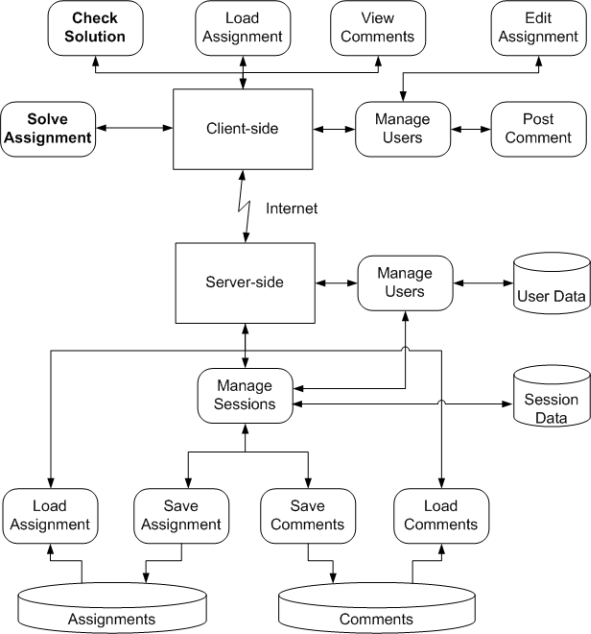
\includegraphics[width=0.85\textwidth]{./img/architecture01a.png}
		\caption{LDBN - System Architecture}
		\label{fig:sysarch}
	\end{center}
\end{figure}

It should be noted that the functions in the diagram represent many classes and 
static methods, which are all serving the same purpose/function. We are not 
going to discuss all 
of the functions in detail, because most of them are straightforward and 
self-explanatory. 
However, in the next section we are going to describe the core package of LDBN,
on which the two most important features of the system depend - 
the \textit{Assignment Solver} and the \textit{Solution Checker}. 
As the names suggest, the 
\textit{Assignment Solver} is used
for giving a sample solution to a given assignment, and the \textit{Solution Checker}
performs series of checks to test the correctness of the given solution.
As we mention in Section~\ref{sec:introldbn}, an assignment consist of a 
relation schema in 1NF. A solution to an assignment consists 
of a decomposition of the schema from 1NF into 2NF, 3NF and BCNF. In addition,
the user must define one of the key candidates of each new relation in each
decomposition. 

Other functions of LDBN include the \textit{Assignemtn Loader}, which loads 
a new assignment from the database. The \textit{Comment Viewer} displays comments for
each assignment, posted by other users. The \textit{User Manager} 
allows unregistered users to create new account and registered users to login with 
their password and username. After users have logged in, they receive an unique 
session id from the server, which allows them to post comments and to use the 
\textit{Assignment Editor}. The \textit{Assignment Editor} provides users with 
the ability to create, edit, save, export and import assignments. 

There are also functions on the server-side. One of them is 
the \textit{Load Assignments} function, which retrieves assignment data from the database,
converts it to XML and then sends it back to the client, analog for \textit{Load Comments}.
\textit{Save Assignment} and \textit{Save Comment} are inserting and updating assignment/comment data in the database, but
first information is passed though the \textit{Session Manager}, which ensures that the data
is coming from a registered user. The \textit{Session Manager} is also responsible for creating
a new session, and killing an existing one. We have another \textit{User Management} on the server-side, which
receives its data from the \textit{User Management} on the client side. It is responsible 
for inserting new users into the database and for modifying existing data such as username, password and email.
It needs to have access to the \textit{Session Data}, in order to ensure that an 
user is always logged in,
before he/she atemps to change any user data.    

\section{Core Package}
In this section we are going to discuss the core package of LDBN, in which all 
the algorithms described in Section~\ref{sec:alg} are implemented. 
The package is extensively
used by the \textit{Assignment Solver} and \textit{Solution Checker}, and it is 
an essential part of LDBN. Figure~\ref{fig:coreuml} shows an UML class diagram
of the most important classes and methods of the package. 

\begin{figure}[h]
	\begin{center}
		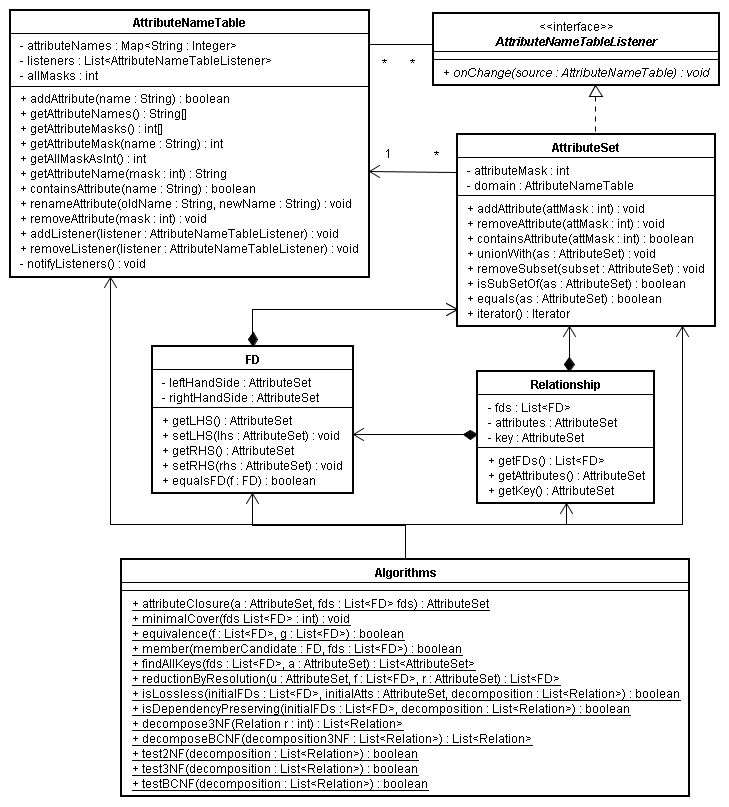
\includegraphics[width=0.9\textwidth]{./img/uml02.png}
		\caption{LDBN - Core Classes}
		\label{fig:coreuml}
	\end{center}
\end{figure}

The \textit{AttributeSet} is a fundamental class in LDBN. 
It holds the attributes of a relationship, which can be used
for many purposes. For instance as the left-hand and right-hand side (LHS and RHS) 
of a functional dependency (FD), or as a set of key attributes. 
In the early stages of the implementation of LDBN, attribute sets
were simply represented as arrays of strings. However, this has proven to be very
inefficient even for trivial operations like comparation or union of two sets. This could 
lead to efficiency problems with
bigger assignments, especially in a single thread environment like JavaScript. 
The solution was to use a variable of type integer as a representation of an entire
attribute set. 
This way attributes are added or removed from the set by using the bit operators, 
thus every attribute is 
a bit index in the integer variable. This has the disadvantage that
assignments can contain only up to 32 attributes, but exceeding 32 attribute 
is highly unlikely to happen in an educational software. On the other side, the 
advantages are of much greater value, as set operations, which are used quite 
often, are performed in almost constant time, since we are using bit operators only.
For example, if we want to make the union of two sets, we just use the 
bitwise OR operation on both integer variables.
 
Every \textit{AttributeSet} object has an associated domain name space called 
\textit{AttributeNameTable}. 
It contains a map, so that the string name of an attribute is mapped to its 
integer representation. In this way information is never lost. It is worth mentioning 
that initially a long variable was used
instead of an integer. This gave us 64 possible attributes in an assignment, 
however, JavaScript has only one numeric data type, which is the double. 
Double has only 53 bits of precision, thus if one want a "real" long integer with 64 bit, 
it has to be emulated. This could hurt the performance of an application~\cite{wgio1}, 
therefore we switched to integers in LDBN. The \textit{AttributeNameTable}
class uses the Event Listener design pattern, as a result of which classes implementing 
the \textit{AttributeNameTableListner} interface can update their content,
whenever changes in the \textit{AttributeNameTable} occur. This is used by instances of the 
\textit{AttributeSet} class, but also by some UI classes. The \textit{FD} class is basically a composition of two \textit{AttributeSets}, 
each one representing the LHS and RHS of the FD. The \textit{Relationship} class holds a relationship, which consists of attributes, 
list of FDs and a key. The \textit{Algorithm} class contains all the algorithms as
static functions. Some of the algorithms have exponential complexity in the worst
case, therefore a lot of the produced output is being cached. This increases the
memory usage, but it could make the application respond much quicker, which
in our opinion is more important for the user.    

\section{User Interface}
It possible to define tow distinct user groups, warranting at least two different
user interfaces for LDBN.  One group would include the lecturers, who will
focus their attention on creating assignments. The other group would be the 
students, who will use the leaning environment mostly for solving 
the assignments provided by the lecturers. It should be noted, that every registered
user can create assignments, thus students can take the role of lecturers as well.
The most important part of a system for end users and critical for system 
success is the UI~\cite{p9}, therefore we tried to provide both 
user groups with fast and easy to use UI. In order to achieve this we put a lot
of our attention in finding a good layout for the UI. The requirements for
the layout were to give the user as much information possible about an 
assignment without loosing the general view. In order to achieve this goal  
we split the UI in four different views using tabs:

\begin{description}
	\item[Home] view is where the users can login, register and view some information 
	about the learning environment.
	\item[Solve Assignment] view is where students can load an assignment, give and
	test their solution. In case they have troubles finding a right solution
	LDBN could generate a sample one and present it.  
	\item[Create Assignment] view is used by lecturers to create, edit, export or import
	assignments.  
	\item[License] view displays a license information about LDBN.
\end{description} 

Furthermore, the \textit{Solve Assignment} view contains the following fields:

\begin{itemize}
	\item Given attributes.
	\item Given FDs.
	\item Minimal Cover.
	\item 2NF, 3NF, BCNF Decomposition.
	\item Comments.
\end{itemize}

The \textit{Given Attitibutes} and the \textit{Given FDs} fields are not editable
and they correspond	to the information stored in each assignment, which is all the 
attributes and all the FDs of a database schema in 1NF. In all other fields 
the the content can be modified by the user.
In the \textit{Minimal Cover} field the user has to define a set of FDs
which are building a minimal (canonical) cover of the \textit{Given FDs}. 
This field is intended to be an intermediate step, which will help the user find easier a right decomposition
in the \textit{2NF, 3NF and BCNF Decomposition} fields. Those last three fields all
work the same way, but the alogotithms for checking the correnctnes of the 
decomposition are different.  
In each decomposition field the user can define a new
relation by assigning attributes, FDs and a key candidate to it. All the relations
within a filed represent a decomposition. Different editors are provided to the users,
such as
the \textit{Attribute Editor}, the \textit{Key Editor} and the \textit{FD Editor}.
The FD Editor is shown in Figure~\ref{fig:fdedit}. Each editor has one or two
text boxes, where users can input names of attributes, in order to 
add or to modify relations, FDs or keys. Furthermore,
each of the editors is wrapped in a draggable dialog window. 
This way the editors do not require any space on any of the fields, 
and can be open only when they are needed.
In addition to this, every attribute and every FD in every field can be dragged and
dropped in the text box of each editor, as a result of which the attributes/FDs
are automatically inserted in the text areas of the editor.
This can help user define attributes, keys or
FDs much quicker, which on the other hand can help improve the usability of 
the learning environment. 
Another useful feature, which also improves the usability of LDBN and greatly reduces
the time for defining relations, 
is the ability to 
import entire decompositions from the 2NF into the 3NF field, and from the 
3NF field into the BCNF field. This was done, because usually 
the differences between the decompositions are not huge, and each decomposition
can be used as a good staring point for the other ones.	
The last field of the \textit{Solve Assignemtn} view is the \textit{Comment} field, 
where users can view and post textual comments on every assignment.
\newline

\begin{figure}[h]
	\begin{center}
		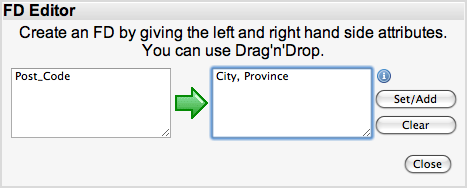
\includegraphics[width=0.6\textwidth]{./img/screen04.png}
		\caption{FD Editor Dialog}
		\label{fig:fdedit}
	\end{center}
\end{figure}

The \textit{Create Assignment} view looks very similar to the 
\textit{Solve Assignment} view. It also has a \textit{Given Attributes} and 
\textit{Given FDs} fields. However, in this view these fields
can be edited using the \textit{Attribute Editor} and the \textit{FD Editor}. 
This allows users to define new assignments or modify existing ones. This view
also allows users to save the assignments in the database or to export them as XML
files to the local file system. Importing an assignment form a XML file is also 
possible.  

In case the user needs help with certain aspects of LDBN, the system provides 
help dialogs for every key feature of the UI. The dialogs can be open
using information buttons (
\includegraphics[scale=0.5]{./img/info.png}), which can be
found near every button or in every editor. This way help information is 
visually organized and the user has fast access to it.

\section{Server-side}
The server-side is mainly used for persistent storage of assignments, user comments,
user and session data. The communication between the web server and the client
is done using the POST method of the Hypertext Transfer Protocol - HTTP/1.1~\cite{w6}.
The POST method has two advantages over the GET method. First, it is more secure, i.e., 
the GET method is defined as safe, which means it is intended only for information 
retrieval and should not change the state of the server. Second, although the
RFC 2616, "Hypertext Transfer Protocol -- HTTP/1.1"~\cite{w6} does not specify
any requirement for URL length, many browsers like Internet Explorer limit
the length of an URL to a maximum of 2048 characters. This length may not be 
enough for LDBN, as it sometimes sends very large assignments back to the server.  

The web server uses XML to send data back to the client. LDBN defines its own XML data
exchange format. The format has several types:

\begin{description}
	\item[Message] for sending string messages, which appear in an alert window on 
	the client-side. Such messages can be for instance an error messages returned
	by the database. 
	\item[Comments] for sending user comments. 
	\item[Session] contains session data for logged in users such as an unique session 
	ID, generated by the server and stored in the database. The ID is used for
	legitimizing user actions on the server-side.
	\item[Assignment List] for sending back meta data for each assignment. This
	information is used by the \textit{Assignment Loader}, in order to display a list
	of all available assignments in the database.
	\item[Assignment] contains a LDBN assignment. 
\end{description}  

\section{Security Issues}
The system uses HTTP 1.1 for the communication between the client and the web
server. This can easily be secured by using HTTPS instead. The upgrade only
require changes to the configuration of the web server. However, using an encrypted
connection does not prevent web applications from SQL injection and cross-site 
scripting attacks. SQL Injection refers to the technique of 
inserting SQL statements into web-based input fields in 
order to manipulate the execution of the SQL queries. Cross Site Scripting 
attacks work by embedding script tags into the web pages. 

Here follows a short example of a SQL injection.
Assuming that we have a poorly implemented PHP script for loading an assignment,
which has the following line of code in it:

\begin{verbatim}
     $sql_statement := "SELECT * FROM assignment WHERE id=$_GET['id'] ";
\end{verbatim}

\noindent If the "id" argument of the GET method is crafted in a specific way by a 
malicious user, the SQL statement may do more than the code author intended. 
For example, setting the "id" argument as:

\begin{verbatim}
     1; DROP TABLE users;
\end{verbatim}

\noindent yields the following SQL statement:

\begin{verbatim}
     SELECT * FROM assignment WHERE id=1; DROP TABLE users;
\end{verbatim}

\noindent The statement would cause the deletion of the "users" table. 

In order to prevent SQL injection and cross-site 
scripting attacks LDBN uses regular expressions for validating
user input, and it escapes HTML special characters like \lt and~\gt.
To the best of our knowledge, it is not possible to perform such attacks on LDBN.

Another issue with web-based applications is password protection. LDBN uses the 
MD5~\cite{w7} one-way encryption algorithm for hashing user passwords. 
To authenticate an user, the password presented by him/her is hashed on the client-side, 
then send to the web server and compared with the stored hash in the database. 
This way the actual password of the user is never sent over the network.
